The individual predictions from the acoustic and the lexical model need to be combined to obtain a final, overall prediction.
Therefore, we fuse the predictions of the two models.
We implemented two different fusion approaches:
The first approach is called \emph{Threshold Fusion}, the second one is called \emph{Balance Fusion}.
The two fusion approaches and the evaluation will be presented in the remainder of this section.

\subsection{Threshold Fusion}
The main idea of the threshold fusion is the following: If the probability for the class \textsc{Period} from the acoustic model is over a certain threshold and the probability for the class \textsc{None} from the lexical model is below a certain threshold, we want to predict a period or a comma.
If the condition is satisfied, the probability of the class \textsc{Period} from the acoustic model is added to the probabilities of the classes \textsc{Period} and \textsc{Comma} from the lexical model.
The idea of the threshold fusion is shown in the Figure~\ref{fig:fusion_1}.
\begin{figure}[ht]
    \centering
    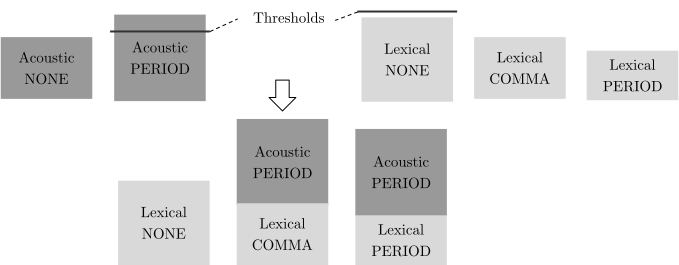
\includegraphics[width=0.7\textwidth]{img/fusion_1.pdf}
    \caption{Threshold Fusion: The probability of the class \textsc{Period} from the acoustic model is added to the probabilities of the classes \textsc{Period} and \textsc{Comma} from the lexical model, if the probability for the class \textsc{Period} from the acoustic model is over a certain threshold and the probability for the class \textsc{None} from the lexical model is below a certain threshold.}
    \label{fig:fusion_1}
\end{figure}
If the condition does not hold, we just take the prediction probabilities of the lexical model as the final predictions.
Thus, the threshold fusion trusts the lexical model more than the acoustic model.
The acoustic model is only taken into account, if the acoustic model is quite certain, that there should be a period, and the lexical model is not certain enough, that there should be no punctuation at all.
In the end, the class with the highest probability is chosen.
For the example in Figure~\ref{fig:fusion_1}, we would predict a comma.

\subsection{Balance Fusion}
The balance fusion sums up weighted probabilities of both models.
Figure~\ref{fig:fusion_2} shows an example.
\begin{figure}[ht]
    \centering
    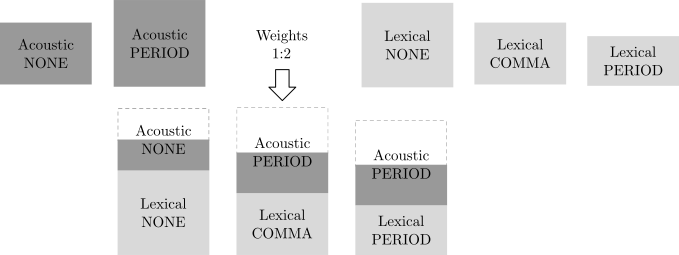
\includegraphics[width=0.7\textwidth]{img/fusion_2.pdf}
    \caption{Balance Fusion: Sum up the weighted probabilities of both models.}
    \label{fig:fusion_2}
\end{figure}
Using weights we can regulate, which model we trust more.
In the example shown in Figure~\ref{fig:fusion_2}, the lexical model is more important than the acoustic model.
In the end, the class with the overall highest probability is chosen again.
So in the example, this would be the class \textsc{None}.

\subsection{Evaluation}
We evaluate both fusion approaches to determine which of them leads to better results.
The evaluation was done on the TED talk data set, because the acoustic model needs the information about the energy and pitch levels and therefore audio files.
We used the \texttt{.ctm} files along with their corresponding \texttt{.sph} file.
Thus, we only have a gold standard for the class \textsc{Period}.
Consequently, the evaluation was only done for this class.

To evaluate the fusion approaches, we remove all sentence boundaries from the data and pass the data on to the lexical and acoustic model.
We chose the best lexical and acoustic model from the previous sections to predict the punctuations.
The predictions from the lexical and acoustic model are then fused.
Therefore, we tested the threshold fusion with different threshold values and the balanced fusion with multiple weights.
Also, we added a baseline fusion for the lexical and acoustic model, which pass on the predictions from the corresponding model.
The predictions returned by the different fusion approaches are then evaluated using the gold standard.
The F-score was used as evaluation metric.
Figure~\ref{fig:eval_fusion} shows the results.

% Remove baseline lexical? No. Rename audio to acoustic? Done.
\begin{figure}[ht]
    \centering
    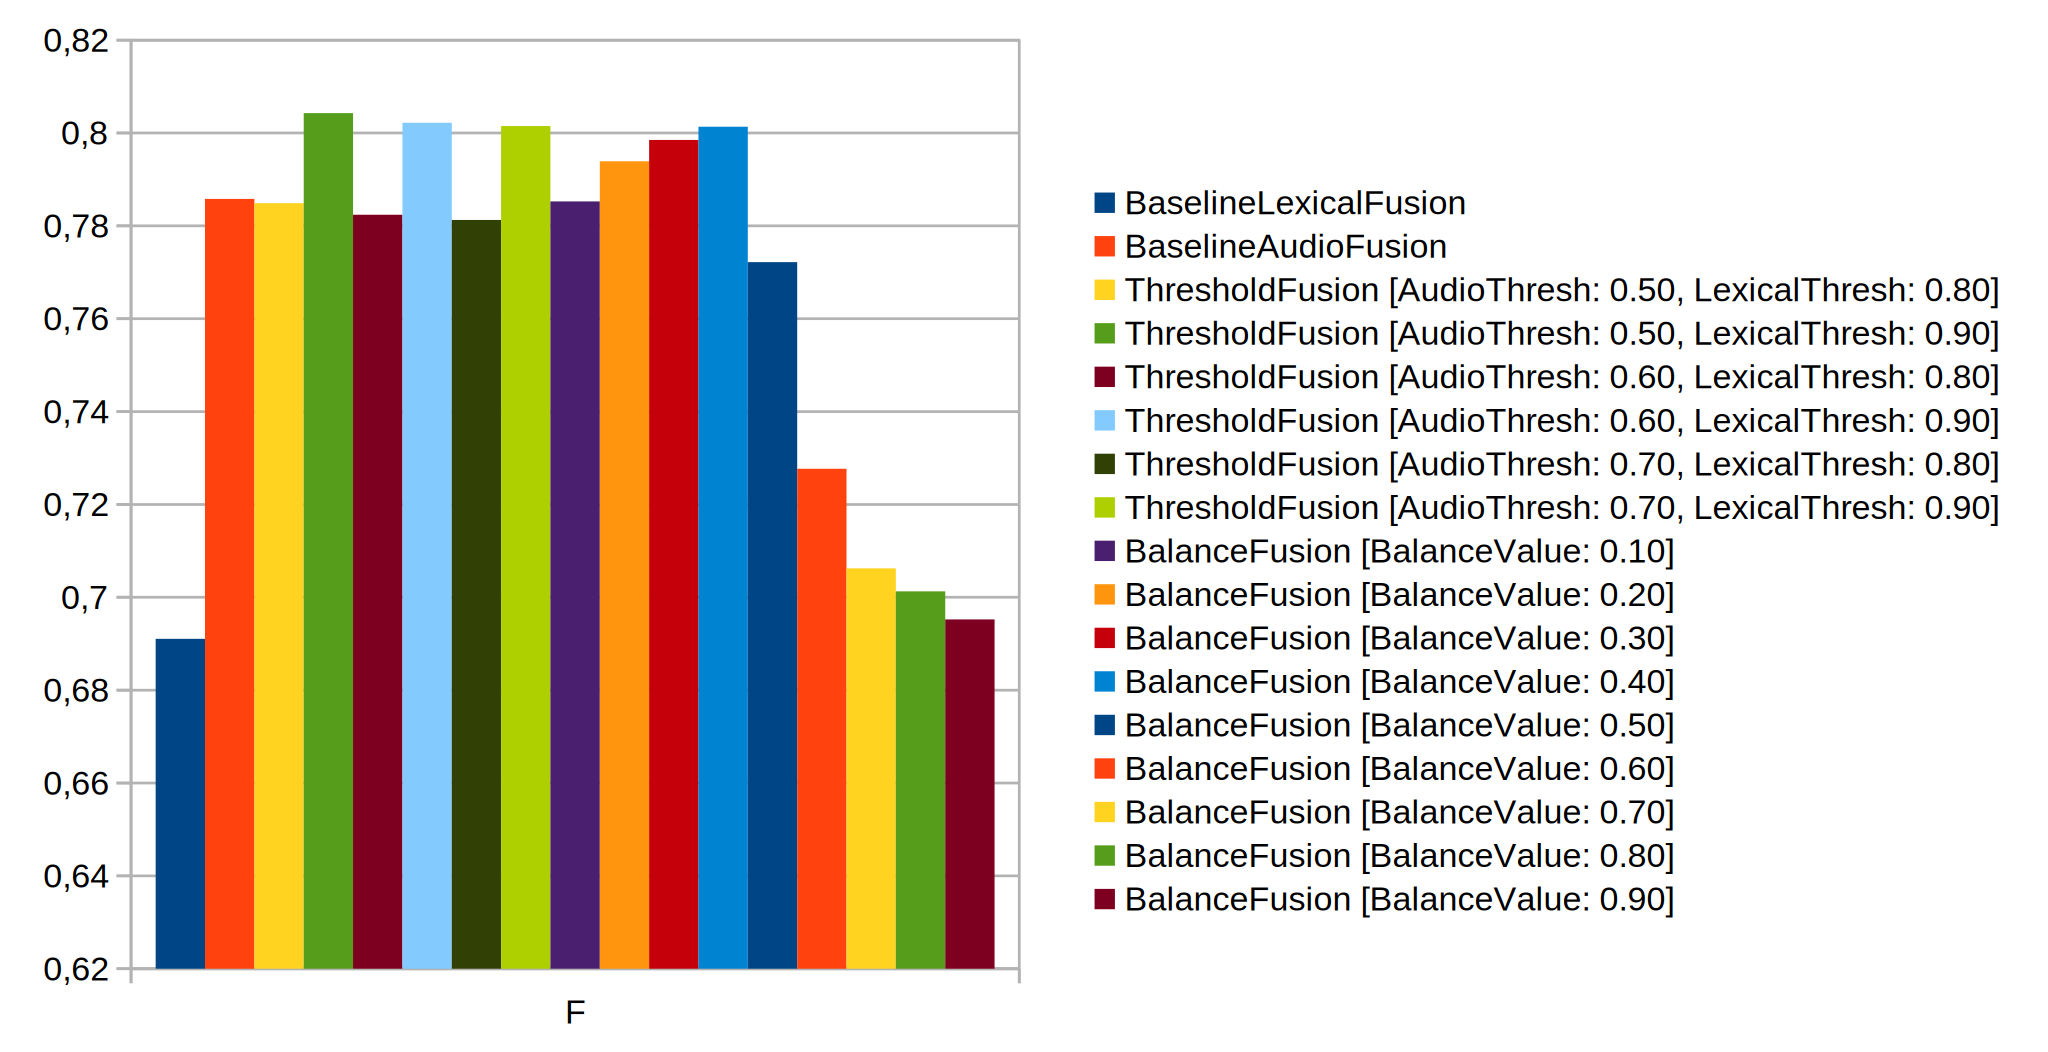
\includegraphics[width=0.7\textwidth]{img/fusion_eval.pdf}
    \caption{Evaluation results for different fusion approaches: The best result is obtained by the threshold fusion with an acoustic threshold of 0.5 and a lexical threshold of 0.9.}
    \label{fig:eval_fusion}
\end{figure}

Because we only have a gold standard for the class \textsc{Period}, the baseline is the F-score from the acoustic model.
Six fusion approaches outperform the F-score of the baseline.
The best one is the threshold fusion with an acoustic threshold of 0.5 and a lexical threshold of 0.9.
It obtained an F-score of 80.43\%, whereas the baseline has an F-score of 78.49\%.
Consequently, fusing the results increases the overall performance.
